\paragraph{\trDistinguishedBasis{}。}\label{sub:distinguished-bases}
下面我们专门讨论底为\trDisk{} $S=D$ 的那些\trExact\trLefschetzFibration。取定一个基点 $*\in S\setminus\mathrm{Critv}(\pi)$，我们愿意把它想象成位于边界上或紧靠边界之处。这意味着，当 $*\notin\partial S$ 时，我们还要额外选取一条\trEmbedding{}的\textbf{\trBasePath}（base path）$\chi\colon[0;1]\to S\setminus\mathrm{Critv}(\pi)$，它从 $\chi(0)=*$ 通到某点 $\chi(1)\in\partial S$。
所谓\trVanishingPath{}的\textbf{\trDistinguishedBasis}（distinguished basis），是指一个由始于 $*$ 的\trVanishingPath{}组成的有序族 $\boldsymbol{\gamma}=(\gamma_1,\ldots,\gamma_m)$，其中 $m=|\mathrm{Critv}(\pi)|$，使得下列条件成立：
\begin{itemize}
\item 诸 $\gamma_k$ 彼此只在 $*$ 处相交，并且它们的出发方向 $\RR^+\cdot\gamma_k'(0)\subset TS_*$ 应当两两不同。
\item 若 $*\in\partial S$，则可以把诸 $\RR^+\cdot\gamma_k'(0)$ 看成\trUpperHalfPlane{}$H$ 中的\trRadial{}半直线，从而它们带有一个自然的\emph{顺时针}次序；规则是：这个次序应与诸 $\gamma_k$ 在 $\boldsymbol{\gamma}$ 中的排序一致。在另一种情形 $*\notin\partial S$，则要求每条 $\gamma_k$ 与 $\chi$ 只在 $*$ 处相交，并且 $\RR^+\cdot\gamma_k'(0)\neq\RR^+\cdot\chi'(0)$。此时，诸 $\RR^+\cdot\gamma_k'(0)$ 便是割缝平面 $\CC\setminus\RR^+$ 中的\trRadial{}半直线，这里被割去的方向即 $\chi'(0)$ 的方向。由此得到一个次序，我们施加与前面相同的条件。
\end{itemize}
所有可能的\trIsotopy{}基类所成的集合带有\trBraidGroup{} $\mathrm{Br}_m$ 的一个作用，它通过所谓的\textbf{\trHurwitz{}移动}（Hurwitz move）实现：第 $k$ 个标准\trGenerator{} $\beta_k$（$1\le k<m$）对应于第 $k$ 个初等 \trHurwitz{}移动 $\boldsymbol{\gamma}\mapsto\boldsymbol{\delta}=\mathscr{L}_k\boldsymbol{\gamma}$。这个移动几乎使所有路径都保持不变，即 $\delta_j=\gamma_j$（$j\neq k,k+1$），而把剩下的两条变成\cref{fig:hurwitz-move}所示的样子。容易验证\trBraidGroup{}关系成立。
\begin{figure}[htbp]
\centering
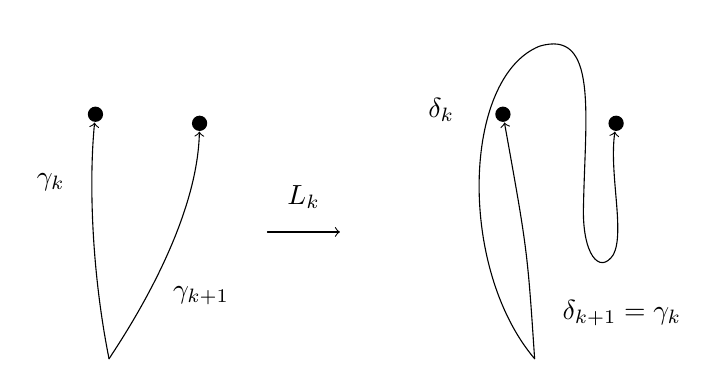
\begin{tikzpicture}[line cap=round,line join=round,scale=1.15]
\fill (-0.15,2.7) circle (2.4pt);%
\fill (1.0,2.6) circle (2.4pt);%
\draw[->,shorten >=3pt] (0,0) .. controls (-0.2,1.0) and (-0.22,2.0) .. (-0.15,2.7);
\node[anchor=east] at (-0.38,1.95) {$\gamma_k$};
\draw[->,shorten >=3pt] (0,0) .. controls (0.5,0.75) and (0.98,1.7) .. (1.0,2.6);
\node[anchor=west] at (0.6,0.7) {$\gamma_{k+1}$};
\draw[->] (1.75,1.4) -- (2.55,1.4);
\node[anchor=south] at (2.15,1.55) {$\mathscr{L}_k$};
\begin{scope}[xshift=4.6cm]
\fill (-0.25,2.7) circle (2.4pt);
\fill (1.0,2.6) circle (2.4pt);
\draw[->,shorten >=3pt] (0.1,0) .. controls (0.02,1.2) .. (-0.25,2.7);
\draw (0.1,0) .. controls (-0.75,1.0) and (-0.7,3.1) .. (0.15,3.45)
      .. controls (0.8,3.65) and (0.66,2.7) .. (0.64,1.7)
      .. controls (0.62,1.15) and (0.82,0.92) .. (0.97,1.15);
\draw[->,shorten >=3pt] (0.97,1.15) .. controls (1.1,1.4) and (0.92,2.05) .. (1.0,2.6);
\node[anchor=east] at (-0.68,2.75) {$\delta_k$};
\node[anchor=west] at (0.3,0.5) {$\delta_{k+1}=\gamma_k$};
\end{scope}
\end{tikzpicture}
\caption{}\label{fig:hurwitz-move}
\end{figure}
下面是一个有关联但稍有不同的视角。设 $\mathscr{D}\subset\Diff^+(S)$ 是由 $S$ 的那些保向\trDiffeomorphism{}组成的子群，它们在 $*$（以及在\trBasePath{}$\chi$ 上，若适用的话）是恒等的，并且把子集 $\mathrm{Critv}(\pi)$ 映到自身。显然，$\pi_0(\mathscr{D})$ 作用在\trDistinguishedBasis{}的\trIsotopy{}类集合上；利用 $\Diff(S,\partial S)$ 的\trContractible{}性，容易看出这个作用是单可递的。同一类论证还表明 $\pi_0(\mathscr{D})$ \trIsomorphic{}于 $\mathrm{Br}_m$；然而这个\trIsomorphism{}并不\trCanonical，所以要多加一分小心。首先，回想对任何避开 $*$（和 $\chi$）且满足 $\mu^{-1}(\mathrm{Critv}(\pi))=\{-1;1\}$ 的\trEmbedding{}路径 $\mu\colon[-1;1]\to S$，我们可以把它的\textbf{\trHalfTwist}（half-twist）$t_\mu\in\mathscr{D}$ 与之相联：它在 $\mu([-1;1])$ 的一个小邻域之外是恒等的，而其局部性态由\cref{fig:half-twist}刻画。显然，这其中涉及一些选取，但所得的类 $[t_\mu]\in\pi_0(\mathscr{D})$ 是唯一的，并且在 $\mu$ 于相关的路径类内作\trIsotopy{}时不变。给定一个\trDistinguishedBasis{}$\boldsymbol{\gamma}$，把 $\gamma_k$ 的逆与 $\gamma_{k+1}$ 连接起来并磨平折角，就可以定义路径 $\mu_k$（$1\le k<m$）。于是，把标准\trGenerator{} $\beta_k$ 映为沿诸 $\mu_k$ 的\trHalfTwist，便给出一个\trIsomorphism{}$\rho_{\boldsymbol{\gamma}}\colon\mathrm{Br}_m\to\pi_0(\mathscr{D})$。在这个\trIsomorphism{}之下，一个初等移动可以简单地写成
\begin{equation*}
\mathscr{L}_k\boldsymbol{\gamma}=t_{\mu_k}^{-1}(\boldsymbol{\gamma})=\rho_{\boldsymbol{\gamma}}(\beta_k^{-1})(\boldsymbol{\gamma}).
\end{equation*}
\begin{figure}[htbp]
\centering
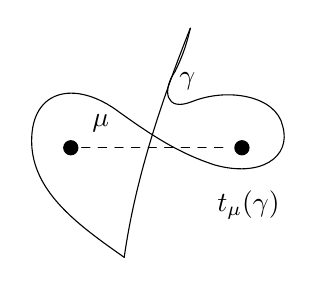
\begin{tikzpicture}[line cap=round,line join=round,scale=1.15]
\draw (0,0) .. controls (0.12,0.85) and (0.4,1.7) .. (0.73,2.53);
\node[anchor=west] at (0.5,1.95) {$\gamma$};
\draw (0,0) .. controls (-0.5,0.35) and (-0.98,0.7) .. (-1.02,1.22)
      .. controls (-1.06,1.85) and (-0.55,1.98) .. (-0.05,1.6)
      .. controls (0.3,1.35) and (0.6,1.15) .. (1.0,1.02)
      .. controls (1.5,0.88) and (1.85,1.1) .. (1.75,1.45)
      .. controls (1.68,1.78) and (1.15,1.88) .. (0.75,1.72)
      .. controls (0.45,1.6) and (0.42,1.85) .. (0.56,2.05)
      .. controls (0.66,2.25) and (0.7,2.4) .. (0.73,2.53);
\fill (-0.59,1.21) circle (2.4pt);
\fill (1.3,1.21) circle (2.4pt);
\draw[dashed] (-0.47,1.21) -- (1.18,1.21);
\node[anchor=south] at (-0.26,1.28) {$\mu$};
\node[anchor=west] at (0.92,0.58) {$t_\mu(\gamma)$};
\end{tikzpicture}
\caption{}\label{fig:half-twist}
\end{figure}
另一方面，这样的移动也会影响 $\rho_{\boldsymbol{\gamma}}$，把它变成一个共轭：
\begin{equation*}
\rho_{\mathscr{L}_k\boldsymbol{\gamma}}(\beta)=t_{\mu_k}^{-1}\circ\rho_{\boldsymbol{\gamma}}(\beta)\circ t_{\mu_k}=\rho_{\boldsymbol{\gamma}}(\beta_k^{-1}\beta\beta_k).
\end{equation*}
把这两个观察结合起来便看出：对所有的 $k_1,\ldots,k_r\in\{1,\ldots,m-1\}$ 与 $\sigma_1,\ldots,\sigma_r\in\{\pm1\}$，都有
\begin{equation*}
\mathscr{L}_{k_r}^{\sigma_r}\ldots\mathscr{L}_{k_1}^{\sigma_1}\boldsymbol{\gamma}=\rho_{\boldsymbol{\gamma}}(\beta_{k_1}^{-\sigma_1}\ldots\beta_{k_r}^{-\sigma_r})(\boldsymbol{\gamma}).
\end{equation*}
用文字来说：元素 $\beta\in\mathrm{Br}_m$ 对一个\trDistinguishedBasis{}$\boldsymbol{\gamma}$ 的作用——它定义为一系列初等移动——与 $\boldsymbol{\gamma}$ 在\trDiffeomorphism{}$\rho_{\boldsymbol{\gamma}}(\beta^{-1})$ 之下的像一致。这特别表明，任何两个基都可以借\trHurwitz{}移动相互联系。
我们现在要为\trVanishingCycle{}引进相应的概念。在一个取定的\trCorneredBoundary{}的\trExactSymplectic\trManifold{}里，考虑 $m$ 个带\trFrame{}的\trExact\trLagrange{}\trSphere{}的有序组 $V=(V_1,\ldots,V_m)$。对把所涉诸\trLagrange{}\trSphere{}作（带\trFrame{}的\trExact{}）\trIsotopy{}而得到的组，我们不加以区分。在这个语境下，初等 \trHurwitz{}移动就是变换 $V\mapsto W=\mathscr{L}_kV$（对某个 $1\le k<m$），由令 $W_j=V_j$（对所有 $j\neq k,k+1$）以及
\begin{equation}\label{eq:hurwitz-move-spheres}
W_k=\tau_{V_k}(V_{k+1}),\qquad W_{k+1}=V_k.
\end{equation}
给出。照常，一般的 \trHurwitz{}移动是指这些变换与其逆的任何\trComposition{}。与前文的联系应当是清楚的：任何\trVanishingPath{}的\trDistinguishedBasis{}$\boldsymbol{\gamma}$ 都决定一个有序组 $V=V_{\boldsymbol{\gamma}}$，它由诸\trVanishingCycle{}$V_k=V_{\gamma_k}$ 构成；这称为相伴的\textbf{\trVanishingCycle{}的\trDistinguishedBasis}（distinguished basis of vanishing cycles）。\cref{thm:vanishing-cycle-piece-transport}与 \eqref{eq:symplectic-picard-lefschetz} 表明，作用在\trVanishingPath{}上的初等 \trHurwitz{}移动 $\mathscr{L}_k$ 诱导出该\trDistinguishedBasis{}的相应移动（在相差\trIsotopy{}的意义下）：
\begin{equation*}
V_{\mathscr{L}_k\boldsymbol{\gamma}}\simeq\mathscr{L}_kV_{\boldsymbol{\gamma}}.
\end{equation*}
定义各组 $V$ 的\textbf{\trHurwitz{}\trEquivalence}（Hurwitz equivalence）为由 \trHurwitz{}移动与\trIsotopy{}生成的\trEquivalence{}关系。用这种语言来说，结论就是：$V_{\boldsymbol{\gamma}}$ 的 \trHurwitz{}\trEquivalence{}类是\trLefschetzFibration{}的一个\trInvariant（严格说来，是这个\trFibration{}连同基点的选取——以及在必要时\trBasePath{}的选取——的\trInvariant）。在适当的意义下，它在沿\trHorizontal{}边界表现良好的\trDeformation{}——即 \cref{sub:isomorphisms-deformations} 中所定义的那种——之下也保持不变。
